\documentclass[a4paper, 10pt]{article}
\usepackage[margin=1in]{geometry}
\usepackage{amsfonts, amsmath, amssymb, amsthm}
%\usepackage[none]{hyphenat}
\usepackage{fancyhdr} %create a custom header and footer
\usepackage[utf8]{inputenc}
\usepackage{enumitem}
\usepackage[english, main=ukrainian]{babel}
\usepackage{pgfplots}
\usepgfplotslibrary{fillbetween}
\usepackage{tikz}
\usepackage{graphicx}
\usepackage{caption}
\usepackage{float}
\usepackage{physics}
\usepackage[unicode]{hyperref}
\usepgfplotslibrary{polar}
\usepackage{ifthen}
\usetikzlibrary{spy}
\usepackage{bbm}
\usepackage{tikz-cd}
\usepackage{centernot}


\fancyhead{}
\fancyfoot{}
\parindent 0ex
\def\huge{\displaystyle}
\def\rightproof{$\boxed{\Rightarrow}$ }
\def\leftproof{$\boxed{\Leftarrow}$ }

\usepackage{pdfpages}

\newtheoremstyle{theoremdd}% name of the style to be used
  {\topsep}% measure of space to leave above the theorem. E.g.: 3pt
  {\topsep}% measure of space to leave below the theorem. E.g.: 3pt
  {\normalfont}% name of font to use in the body of the theorem
  {0pt}% measure of space to indent
  {\bfseries}% name of head font
  {}% punctuation between head and body
  { }% space after theorem head; " " = normal interword space
  {\thmname{#1}\thmnumber{ #2}\textnormal{\thmnote{ \textbf{#3}\\}}}

\theoremstyle{theoremdd}
\newtheorem{theorem}{Theorem}[subsection]
  
\theoremstyle{theoremdd}
\newtheorem{definition}[theorem]{Definition}

\theoremstyle{theoremdd}
\newtheorem*{definition*}{Definition.}

\theoremstyle{theoremdd}
\newtheorem{samedef}[theorem]{Definition}

\theoremstyle{theoremdd}
\newtheorem{example}[theorem]{Example}

\theoremstyle{theoremdd}
\newtheorem*{example*}{Example.}

\theoremstyle{theoremdd}
\newtheorem*{lemma*}{Lemma.}

\theoremstyle{theoremdd}
\newtheorem*{theorem*}{Theorem.}

\theoremstyle{theoremdd}
\newtheorem{proposition}[theorem]{Proposition}

\theoremstyle{theoremdd}
\newtheorem*{proposition*}{Proposition.}

\theoremstyle{theoremdd}
\newtheorem{remark}[theorem]{Remark}

\theoremstyle{theoremdd}
\newtheorem*{remark*}{Remark.}

\theoremstyle{theoremdd}
\newtheorem{lemma}[theorem]{Lemma}

\theoremstyle{theoremdd}
\newtheorem{corollary}[theorem]{Corollary}

\theoremstyle{theoremdd}
\newtheorem*{corollary*}{Corollary.}

\newenvironment{pf}{\vspace*{-3mm} \textbf{Proof. \\}}{$\blacksquare$}
\newenvironment{pfMI}{\vspace*{-3mm} \textbf{Proof MI. \\}}{$\blacksquare$}
\newenvironment{pfNoTh}{\textbf{Proof. \\}}{$\blacksquare$}

\renewcommand{\qedsymbol}{$\blacksquare$}

\makeatletter
\renewenvironment{proof}[1][Proof.\\]{\par
\pushQED{\hfill \qed}%
\normalfont \topsep6\p@\@plus6\p@\relax
\trivlist
\item\relax
{\bfseries
#1\@addpunct{.}}\hspace\labelsep\ignorespaces
}{%
\popQED\endtrivlist\@endpefalse
}
\makeatother

\newcommand{\notiff}{%
  \mathrel{{\ooalign{\hidewidth$\not\phantom{"}$\hidewidth\cr$\iff$}}}}

\DeclareMathOperator{\ord}{ord}
\DeclareMathOperator{\Mat}{Mat}
\DeclareMathOperator{\card}{card}
\DeclareMathOperator{\charac}{char}
\DeclareMathOperator{\coker}{coker}
\DeclareMathOperator{\id}{id}
\DeclareMathOperator{\lcm}{lcm}
\DeclareMathOperator{\linspan}{span}
\DeclareMathOperator{\Cl}{Cl}
\DeclareMathOperator{\Int}{Int}
\DeclareMathOperator{\diam}{diam}

\newcommand\thref[1]{\textbf{Th.~\ref{#1}}}
\newcommand\defref[1]{\textbf{Def.~\ref{#1}}}
\newcommand\exref[1]{\textbf{Ex.~\ref{#1}}}
\newcommand\prpref[1]{\textbf{Prp.~\ref{#1}}}
\newcommand\rmref[1]{\textbf{Rm.~\ref{#1}}}
\newcommand\lmref[1]{\textbf{Lm.~\ref{#1}}}
\newcommand\crlref[1]{\textbf{Crl.~\ref{#1}}}
%\renewcommand{\stcomp}[1]{{#1}^{\mathsf{c}}}

\newcommand{\eqbydef}{\overset{\text{def.}}{=}}
\newcommand\homom[2]{\text{Hom}({#1},{#2})}
\newcommand{\symdif}{\,\triangle\,} % symmetric difference
\newcommand\End[1]{\text{End}({#1})}
\newcommand\Aut[1]{\text{Aut}({#1})}
\newcommand\Orb{\text{Orb}}
\newcommand\Stab{\text{Stab}}
\newcommand\ncl{\text{ncl}}

%delete

\begin{document}
\section{Гомотопія петель}
\newpage
\section{Гомологія}
Головна мотивація: відрізняти топологічні простори на наявність 'дір'. Поняття 'діри' доволі специфічне та має різні розмірності.\\
Наприклад, розглянемо в стандартному розумінні 'діру' на наступному малюнку.
\begin{figure}[H]
\centering
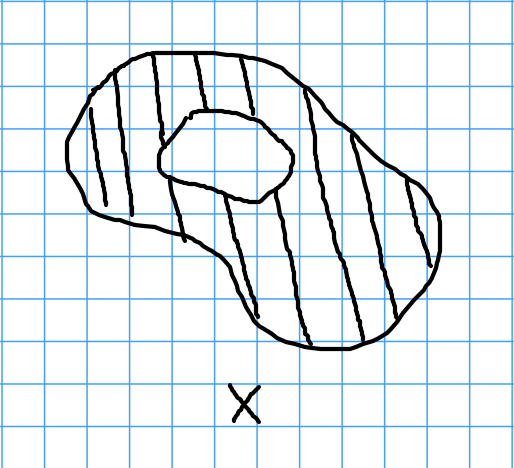
\includegraphics[scale=0.25]{space_with_one_dimensional_hole.png}
\end{figure}
Це приклад так званої $1$-вимірної діри. Це можна сприймати як \textit{цикл}, який не обмежує \textit{$2$-вимірну область} в цьому просторі. Таку ж ідею поняття 'діри' можна повторити на більшу розмірність.\\
Зокрема тепер розглянемо сферу $S^2$. Одразу скажу, що $1$-вимірних дір нема там зовсім (як би ми там не будували цикл, ми обмежуємо $2$-вимірну область).\\
Всередині приклад так званої $2$-вимірної діри. Це можна сприймати як \textit{поверхню}, який не обмежує \textit{$3$-вимірну область} в цьому просторі. Воно не видно очами, але всередині сфери заповнили повітрям, тому це тіпа $2$-вимірна 'діра'.\\
Що таке $3$-вимірна 'діра', $4$-вимірна 'діра' тощо узагальнимо пізніше.
\bigskip \\
Тепер глянемо на тор $T$. Там є одна $2$-вимірна діра та аж дві $1$-вимірних дір.

\subsection{Симплиційна гомологія}
Ідея полягає в тому, щоб спочатку наш простір розбити на так звані симплекси ($0$-симплекс -- точка, $1$-симплекс -- відрізок, $2$-симплекс -- трикутник, $3$-симплекс -- тетраедр, а далі узагальнення зрозуміле).\\
Наприклад, маємо коло $S^1$. Його можна побудувати за допомогою одного $0$-симплекса та одного $1$-симплекса. Навчимося рахувати так звані границі $\partial$ від $1$-симплекса.\\
$\partial([a,b]) = [b] - [a]$.\\
Тобто це, по суті, різниця кінцевих точок (які є $0$-симплексами). Зокрема для кола $S^1$ там є один $1$-симплекс $[a,a]$, причому $\partial([a,a]) = 0$. Зв'яжемо алгебру з геометрією. Візуально бачимо цикл, а алгебраїчно це означає, що $\partial \text{цикл} = 0$. Отже, $\ker \partial$ -- колекція циклів.\\
Однак у нас можуть бути цикли, що є дірами так й цикли, що не є дірами. Треба їх якось відрізняти. Для цього ми будемо брати фактор $\ker \partial$ по деякій іншій множині.

\subsection{Сингулярна гомологія}
Її тільки використовувати для побудови теорії. Таке рахувати просто неможливо!\\
Водночас симпліційною гомологією важко будувати теорію. Але легко рахувати її.\\
\bigskip \\
Насправді, сингулярна гомологія та симплиційна гомологія дають ізоморфізм.

\subsection{Відносна група гомологій}
Є функція $\pmod n$, яка ігнорує всі множники $n$. Ми прибираємо зайву інформацію таким чином.\\
Схожим чином працює відносна гомологія, де ми ігноруємо всі сингулярні ланцюги, які в підмножині деякої множини.\\
$H_n(X,A)$ -- гомологія $X$ за модулем $A$.
\bigskip \\
Для чого? Це нам допоможе знайти $H_n(X/_A)$. А точніше зв'язок з $H_n(X),H_n(A),H_n(X/_A)$.
\end{document}